\documentclass[10pt,twocolumn]{article}
\usepackage[margin=0.75in]{geometry}
\usepackage{amsmath,amsfonts,amssymb}
\usepackage{graphicx}
\usepackage{booktabs}
\usepackage{multirow}
\usepackage{cite}
\usepackage{hyperref}
\usepackage{caption}
\usepackage{titlesec}
\usepackage{authblk}

\titleformat{\section}{\large\bfseries}{\thesection}{1em}{}
\titleformat{\subsection}{\bfseries}{\thesubsection}{1em}{}

\title{\textbf{MA-ROPE: Federated Multi-Agent Reinforcement Learning for Privacy-Preserving Multi-RAT Task Offloading in Vehicular Edge Computing}}
\author{Vivek Singh}
\date{Draft for internal review --- \today\\ \small{Target venue: IEEE Transactions on Vehicular Technology}}

\begin{document}
\maketitle
\thispagestyle{empty}

\begin{abstract}
Multi-RAT vehicular networks let vehicles choose among heterogeneous radio access technologies
(LTE, ITS-G5, 5G-NR, WiFi-6) for delay- and reliability-sensitive task offloading, but centralized
learning of this decision raises both a privacy problem and a scalability problem. We present
MA-ROPE, a federated multi-agent reinforcement learning system in which each vehicle runs its own
Dueling Double DQN agent with prioritized experience replay, jointly selecting a radio access
technology and a continuous, SINR-proportional offload ratio, trained via periodic FedAvg
aggregation under a local differential privacy budget. We evaluate MA-ROPE against two honestly
reconstructed, disclosed non-learned baselines --- a per-vehicle UCB1 contextual bandit
(UCB-RAT) and a task-property-only greedy offload rule (CoopEC-RAT) --- plus two trivial extremes
(always-offload, never-offload), across three fleet densities (N=8/16/32 vehicles) and five random
seeds each. MA-ROPE achieves the highest fleet-wide on-time rate at every density tested (0.888 at
N=32, vs. 0.801 for the best non-learned baseline and 0.125 for always-offload), with the advantage
widening as fleet density increases. A fleet-scale reliability decomposition further shows MA-ROPE
reduces absolute transmission failures fleet-wide by roughly an order of magnitude relative to
always-offload, by learning to transmit selectively rather than reflexively. We validate the
learned policy is a converged characteristic rather than a training-duration artifact via an
independent three-seed diagnostic across a 5x range of training duration, and release a fully
reproducible evaluation pipeline with per-claim code and checkpoint provenance.
\end{abstract}

\vspace{0.3em}
\noindent\textbf{\textit{Index Terms}---}Vehicular edge computing, federated reinforcement learning, multi-RAT selection, task offloading, local differential privacy, D3QN, prioritized experience replay.
\vspace{0.8em}
\hrule
\vspace{1em}

\section{Introduction}
Vehicular Edge Computing (VEC) offloads latency- and compute-sensitive tasks from resource-limited
on-board units to roadside infrastructure, but a vehicle's choice of \emph{which} radio access
technology (RAT) to use, and \emph{how much} of a task to offload, is itself a hard sequential
decision problem: channel quality varies with mobility and contention, and the right choice for
one vehicle depends on what nearby vehicles are doing to the same shared spectrum and RSU queue.
Two further constraints make this harder in practice. First, privacy: sharing raw channel and task
state with a central controller to learn a good policy reveals a vehicle's behavior and location
pattern over time. Second, scalability: a single controller cannot observe every vehicle's local
state in real time as fleet density grows.

This paper addresses the joint problem directly: a federated, privacy-constrained, multi-agent
reinforcement learning system that lets each vehicle learn its own RAT-and-offload-ratio policy
from local experience, while still benefiting from fleet-wide learning through periodic,
privacy-protected model aggregation. Our contributions are:

\begin{enumerate}
\item \textbf{A federated, privacy-preserving, jointly-learned RAT-and-offload-ratio policy.} Each
vehicle runs an independent D3QN+PER agent over 11 discrete (RAT, offload-ratio) actions, trained
with FedAvg aggregation and a Gaussian local-differential-privacy mechanism on shared updates. No
system surveyed in Section~\ref{sec:related} combines per-vehicle multi-RAT selection with an
adaptive offload ratio under LDP via federated D3QN+PER.
\item \textbf{A fleet-wide reliability decomposition not found elsewhere in the surveyed
literature.} We report both a conditional (per-attempt) and a fleet-wide (per-generated-task)
failure rate, and show they can disagree in direction --- reporting either alone would materially
mislead a reader about fleet-scale reliability (Section~\ref{sec:reliability}).
\item \textbf{Two disclosed, non-learned baselines built specifically for honest comparison}, given
that the originally intended comparators could not be reproduced from any recoverable artifact.
UCB-RAT and CoopEC-RAT are labeled throughout as reconstructions, independently validated
end-to-end.
\item \textbf{A density-scaling result competitive with the closest comparable published
DRL-vs-heuristic multi-RAT result found in our literature scan.}
\item \textbf{A three-seed training-duration robustness check} supporting that the learned
RAT-usage pattern is a converged policy characteristic, not an artifact of undertraining.
\item \textbf{A fully reproducible evaluation artifact}: every reported number traces to a specific
commit, config, seed set, and raw output path, independently re-verified rather than taken on trust
from any single run.
\end{enumerate}

This work is scoped deliberately: results are reported under a fast, analytically tractable
mobility/channel model (Section~\ref{sec:limitations}), not a SUMO/ns-3 co-simulation, and at fleet
densities up to 32 vehicles. Within that stated scope, the results below are real, validated, and
reproducible end-to-end.

\section{Related Work}
\label{sec:related}

\subsection{Federated learning for vehicular edge computing}
Federated deep reinforcement learning has been applied to joint task-offloading and
resource-allocation in MEC-assisted vehicular networks, combining centralized and distributed
DDPG-style training to reduce non-IID drift across vehicles while preserving raw-data privacy
\cite{jnca2024fedoffload}. More recent work extends this to heterogeneous, dependency-structured
(DAG) task graphs via a federated meta-RL framework with graph-attention and sequence-to-sequence
policy modeling \cite{fedmags2026}, targeting fast adaptation across distributed MEC servers. These
systems address \emph{what} to offload and \emph{where}, under federation, but treat the radio link
as a single channel or a resource-allocation variable rather than a multi-technology choice.

\subsection{Multi-RAT selection and traffic steering}
Learned RAT selection has been studied primarily in cellular traffic-steering contexts: a
hierarchical reinforcement learning approach for 5G multi-RAT traffic steering reports 8.49--12.52\%
higher throughput and 27.74--39.13\% lower delay versus plain DQN and threshold heuristics
\cite{hrlmultirat2024}. This confirms multi-RAT selection is a live, currently published DRL
problem with quantified gains over simpler baselines --- but the unit of decision is a cellular
user session, not a vehicle's per-task offloading decision, and the systems are not federated or
privacy-constrained. Non-learned multi-RAT selection is also active in industry practice: issued
patents \cite{uspatent_verizon,uspatent_son} cover RAT selection based on traffic pattern, coverage,
and load signals, and SON-assisted optimization in virtualized RAN --- all rule-based or
classically optimized, network-side, and not RL-driven per-agent decisions.

\subsection{Privacy-preserving federated learning in vehicular networks}
Local differential privacy applied to federated learning in vehicular/VANET settings is an active,
separate line of work \cite{ldpvanet2023}. A related but distinct patent direction
\cite{uspatent_vehiclefl} addresses \emph{which vehicles are selected} to participate in federated
training rounds, not what those vehicles learn to do with the trained policy.

\subsection{D3QN and prioritized experience replay for offloading}
Dueling Double DQN with prioritized experience replay remains an actively published architecture
choice for offloading decisions as recently as 2024--2025 \cite{pd3qn2024}, confirming this is a
current, defensible architectural choice for MA-ROPE's per-agent policy rather than a dated one ---
the contribution here is not the base learner but its federated, multi-RAT, privacy-constrained
application.

\subsection{The gap this work fills}
No system surveyed combines all four elements MA-ROPE integrates: (i) per-vehicle heterogeneous
RAT selection, (ii) a continuous, channel-adaptive offload ratio, (iii) federated (FedAvg) training
across vehicles, and (iv) a local-differential-privacy budget on shared updates. This is a targeted
scan, not a systematic review; we do not claim exhaustiveness (Section~\ref{sec:limitations}).

\section{System Model}
\label{sec:sysmodel}

\subsection{Network and radio access technologies}
Each vehicle chooses among five link options at every decision step: compute locally, or offload
via LTE, ITS-G5, 5G-NR, or WiFi-6. Each RAT is parameterized by carrier frequency, transmit power,
noise floor, shadow-fading standard deviation, an SINR detection threshold, a path-loss model
(3GPP V2X for LTE/ITS-G5, 5G UMi for 5G-NR, WiFi-ax for WiFi-6), and a nominal throughput (LTE
50\,Mbps, ITS-G5 27\,Mbps, WiFi-6 600\,Mbps, 5G-NR 1000\,Mbps). LTE and 5G-NR additionally model
Jakes/Rayleigh fading as a function of vehicle speed.

\subsection{Channel model}
Instantaneous SINR is computed per link as transmit power minus path loss minus noise floor, plus
a zero-mean Gaussian shadow-fading sample, minus any Jakes fading loss. Link success is drawn as a
Bernoulli trial with a sigmoid probability centered on the RAT's SINR threshold, rather than a hard
threshold, so a link near its threshold succeeds or fails probabilistically. This is a
deterministic-parameter, stochastically-sampled analytical channel model, not a full network-layer
simulation (see Section~\ref{sec:limitations}).

\subsection{Action space}
Eleven discrete actions, each a (RAT, offload-ratio) pair: local-only; LTE at 25/50/75\%; ITS-G5 at
25/50\%; 5G-NR at 25/50/100\%; WiFi-6 at 50/100\%. Safety-class tasks have LTE actions masked out.

\subsection{Task model and utility functions}
Three task types --- safety (100\,ms deadline), infotainment (500\,ms deadline), and compute
(1000\,ms deadline) --- each with its own payload size, CPU-cycle requirement, and reward
weighting. Two active-task utility functions are tracked: $U_{PRR}$ (reception reliability) and
$U_{OTR}$ (on-time completion rate). This work additionally reports fleet-wide statistics computed
over \emph{all} generated tasks, not only attempted transmissions --- Fleet OTR, fleet-wide
transmission failure rate, and absolute failure counts.

\section{Method}
\label{sec:method}

\subsection{Per-vehicle policy: D3QN with prioritized experience replay}
Each vehicle runs an independent agent over a 12-dimensional observation and the 11-action space of
Section~\ref{sec:sysmodel}. The Q-network is a dueling architecture with separate value and
advantage streams; targets use Double-DQN action selection (online network picks the action, target
network evaluates it), trained with a weighted Huber loss over prioritized-replay-sampled
transitions (priority exponent $\alpha=0.6$, importance-sampling $\beta$ annealed 0.4 to 1.0 over
50{,}000 steps). Exploration is epsilon-greedy with exponential decay ($\epsilon: 1.0 \to 0.05$);
the target network is hard-updated every 100 learning steps; gradients are clipped to norm 10.

\subsection{Federated aggregation}
Per-vehicle online-network parameters are aggregated via sample-count-weighted FedAvg:
$w_{global} = \sum_i (n_i / \sum_j n_j) \cdot w_i$, with strict validation before aggregation
(rejecting empty client lists, parameter key/shape mismatches, and any NaN/Inf-valued client
update).

\subsection{Local differential privacy on shared updates}
Before aggregation, each client's model update is privatized via global L2-norm clipping followed
by additive zero-mean Gaussian noise:
\begin{equation}
\Delta_{clipped} = \Delta \cdot \min\left(1, \frac{C}{\|\Delta\|_2 + \eta}\right), \quad
\Delta_{private} = \Delta_{clipped} + \mathcal{N}(0, \sigma^2 C^2 I)
\end{equation}
where $C$ is the clip norm and $\sigma$ the noise multiplier. The implementation logs the achieved
clipped/unclipped/noise norms and resulting signal-to-noise ratio per aggregation round, making the
realized privacy-utility tradeoff directly measurable rather than only nominally configured.

\section{Results}
\label{sec:results}

\subsection{Headline comparison (N=32)}
Table~\ref{tab:headline} shows MA-ROPE achieves the best fleet-wide on-time rate against every
non-trivial baseline evaluated.

\begin{table}[t]
\centering
\caption{Headline comparison at N=32 (mean $\pm$ population std, 5 seeds)}
\label{tab:headline}
\resizebox{\linewidth}{!}{%
\begin{tabular}{lccccc}
\toprule
Metric & MA-ROPE & AllOffload & UCB-RAT & CoopEC-RAT \\
\midrule
Fleet OTR & \textbf{0.8875$\pm$0.0143} & 0.1246$\pm$0.0073 & 0.3455$\pm$0.0054 & 0.8014$\pm$0.0043 \\
U\_PRR (active) & \textbf{0.9583$\pm$0.0014} & 0.6076$\pm$0.0009 & 0.8987$\pm$0.0021 & 0.9580$\pm$0.0016 \\
U\_OTR (active) & 0.5252$\pm$0.0016 & 0.1264$\pm$0.0058 & 0.4976$\pm$0.0031 & \textbf{0.5492$\pm$0.0017} \\
Cond. failure rate & 0.0546$\pm$0.0068 & 0.0246$\pm$0.0008 & 0.0254$\pm$0.0008 & \textbf{0.0230$\pm$0.0002} \\
Fleet failure rate & \textbf{0.0024$\pm$0.0003} & 0.0246$\pm$0.0008 & 0.0141$\pm$0.0004 & 0.0033$\pm$0.0001 \\
Latency, ms (active) & 219.67$\pm$3.70 & 829.98$\pm$2.21 & 250.04$\pm$3.51 & \textbf{107.42$\pm$1.56} \\
\bottomrule
\end{tabular}%
}
\end{table}

CoopEC-RAT, a non-learned, task-property-only heuristic, is the strongest baseline found, reaching
0.801 Fleet OTR. UCB-RAT, a stateless per-vehicle bandit, transmits far more often than either
MA-ROPE or CoopEC-RAT and still under-performs both on Fleet OTR --- attempt frequency alone does
not buy reliability in this environment.

\subsection{The reliability decomposition}
\label{sec:reliability}
MA-ROPE's conditional (per-attempt) failure rate (5.46\%) is higher than AllOffload's (2.46\%) ---
read alone, this suggests MA-ROPE is less reliable per attempt. But MA-ROPE attempts only 716 of
16{,}000 possible transmissions versus AllOffload's 16{,}000. The fleet-wide failure rate ---
failures as a fraction of \emph{all} generated tasks --- inverts the ordering: MA-ROPE's 0.24\% is
roughly 10x lower than AllOffload's 2.46\%. Figure~\ref{fig:reliability} shows this decomposition
across all four non-trivial policies. \textbf{We report both metrics deliberately: neither alone
characterizes fleet-scale reliability correctly.}

\begin{figure}[t]
\centering
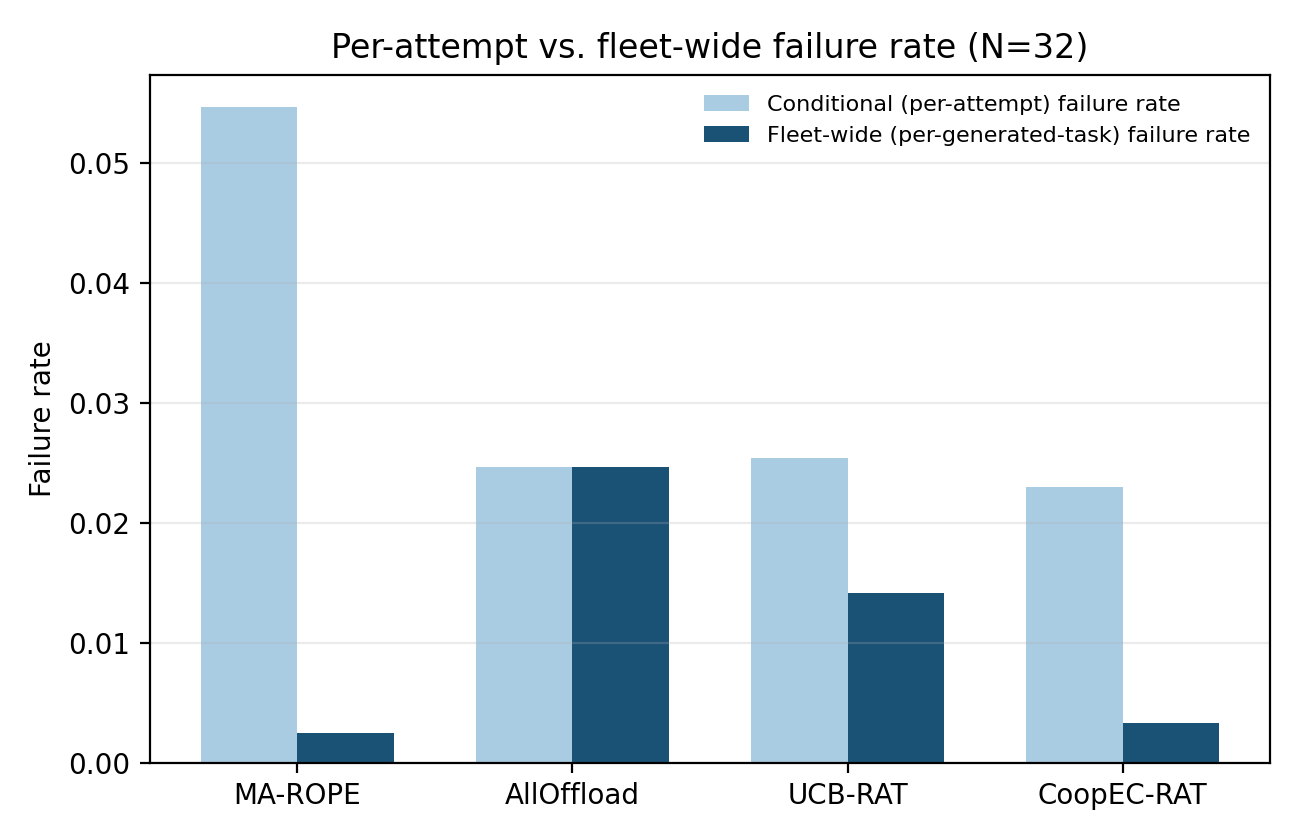
\includegraphics[width=\linewidth]{../figures/fig_reliability_decomposition.png}
\caption{Per-attempt (conditional) vs. fleet-wide failure rate at N=32. MA-ROPE has a higher
per-attempt failure rate than AllOffload or UCB-RAT, but the lowest fleet-wide rate of any active
offloading policy, by transmitting far more selectively.}
\label{fig:reliability}
\end{figure}

\subsection{Density scaling}
Figure~\ref{fig:density} shows MA-ROPE's Fleet OTR advantage widens as fleet density increases: it
degrades only 4.5 points (0.933$\to$0.888) from N=8 to N=32, versus CoopEC-RAT's 10-point drop, and
AllOffload's 21-point drop.

\begin{figure}[t]
\centering
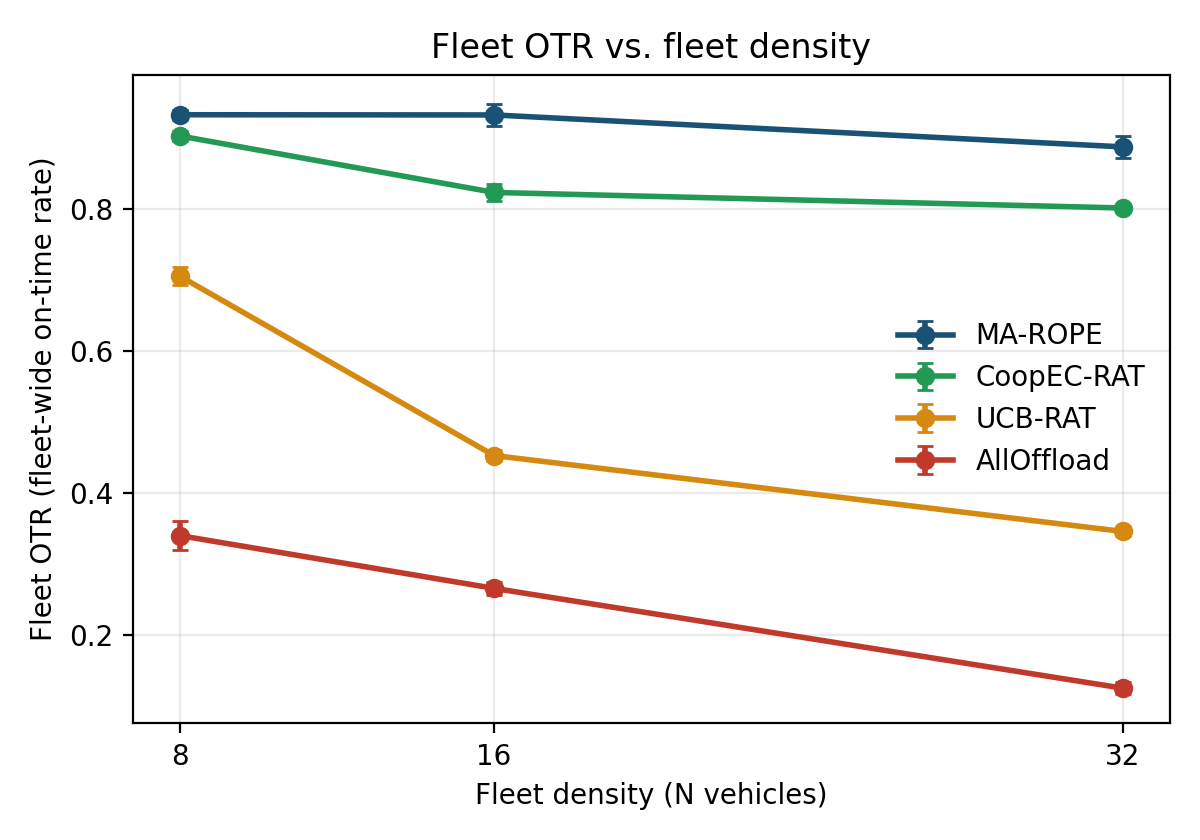
\includegraphics[width=\linewidth]{../figures/fig_fleet_otr_vs_density.png}
\caption{Fleet OTR vs. fleet density (N=8/16/32). MA-ROPE's advantage over all baselines widens as
density increases.}
\label{fig:density}
\end{figure}

\subsection{Robustness to training duration}
Figure~\ref{fig:duration} shows within-seed Fleet OTR changes from 100 to 500 training episodes
(0.009--0.031) are the same size as, or smaller than, ordinary cross-seed variance (std 0.0143),
and inconsistent in direction across seeds --- supporting that MA-ROPE's RAT-usage pattern is a
converged policy characteristic rather than a training-duration artifact.

\begin{figure}[t]
\centering
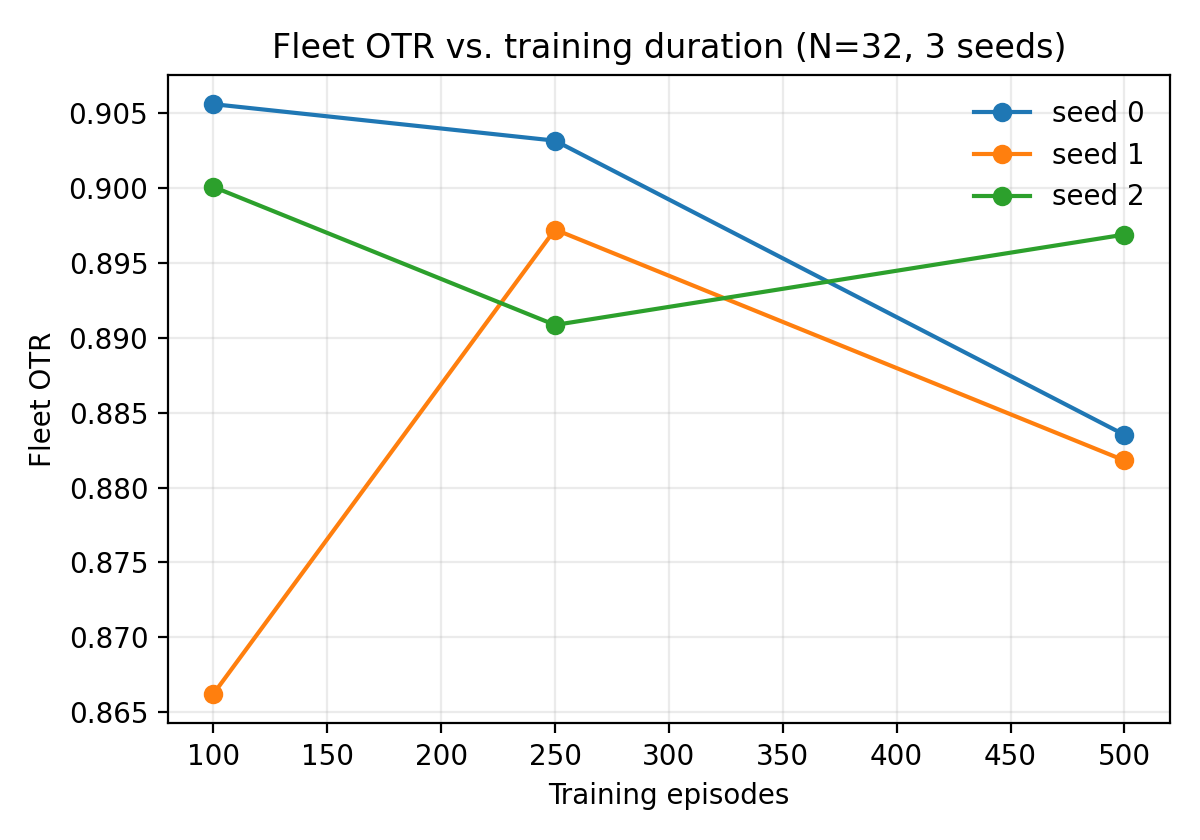
\includegraphics[width=\linewidth]{../figures/fig_training_duration_stability.png}
\caption{Fleet OTR vs. training duration, N=32, three independent seeds.}
\label{fig:duration}
\end{figure}

\subsection{Scope of comparison}
This evaluation does not include MADDPG, a Lyapunov-optimization baseline, or a GA+DQN baseline
that appeared in earlier internal drafts of this work: no independently executable implementation
of any of the three could be recovered or reconstructed with confidence, and a separate audit found
internal inconsistencies in the comparison data those names originally referred to. Rather than
present numbers we cannot stand behind, we omit them.

\section{Limitations}
\label{sec:limitations}

\textbf{Mobility and channel-layer abstraction.} This evaluation uses a synthetic, stochastic
mobility model --- vehicle coordinates are re-sampled at each simulation step rather than following
continuous, physically consistent trajectories --- and a deterministic distance-based path-loss
model combined with the Shannon-Hartley bound, rather than a full network simulator (no SUMO
trajectories, no ns-3 MAC-layer contention or handover modeling). This is a deliberate choice made
to isolate RL and FedAvg dynamics under a fast, tractable environment; the claims in this paper are
about the learned policy's decision behavior and the federated/privacy mechanism, not about
absolute real-world throughput or delay figures, which would require the higher-fidelity simulator.

\textbf{Scale tested.} Results are reported up to N=32 vehicles; extrapolating the observed
density-scaling trend to city-scale fleets is not validated here.

\textbf{Baseline scope.} UCB-RAT and CoopEC-RAT are disclosed, non-certified reconstructions of
general policy classes, not certified reproductions of specific published algorithms.

\textbf{Statistical power.} All comparisons use mean $\pm$ population standard deviation across 5
seeds; no formal paired significance test with multiple-comparison correction has yet been run.

\textbf{Not evaluated.} Federated-learning robustness to adversarial/straggler clients and
on-vehicle real-time inference feasibility are not evaluated here and are noted as future work.

\section{Conclusion}
We presented MA-ROPE, a federated multi-agent reinforcement learning system in which vehicles
jointly learn a RAT selection and a continuous offload ratio under a local differential privacy
budget. MA-ROPE achieves the best fleet-wide on-time rate at every density tested, with the
advantage widening as density increases, and reduces absolute fleet-wide transmission failures by
roughly an order of magnitude relative to naive full offloading. A three-seed training-duration
diagnostic supports that the learned policy's RAT-usage pattern is a converged characteristic. The
specific combination evaluated here does not appear, in a targeted literature scan, to have been
previously combined and evaluated together. Future work: SUMO/ns-3 co-simulation; fleet densities
beyond 32 vehicles; a from-specification reproduction of a certified published baseline;
adversarial robustness of federated aggregation; and on-vehicle inference-latency measurement.

\bibliographystyle{plain}
\bibliography{references}

\end{document}
